\documentclass[12pt]{article}

\usepackage{Homework}

% Creates the header and footer.
\pagestyle{fancy}
\fancyhead[l]{Michael Hoon, $1006617$}
\fancyhead[c]{40.002 Optimisation Problem 2}
\fancyhead[r]{\today}
\fancyfoot[c]{\thepage}
\renewcommand{\headrulewidth}{0.2pt} %Creates a horizontal line underneath the header
\renewcommand{\footrulewidth}{0.2pt}
\setlength{\headheight}{15pt} %Sets enough space for the header
\newcommand{\HRule}[1]{\rule{\linewidth}{#1}}

\begin{document}

\title{ \normalsize \textsc{} 
        \\ [2.0cm]
		\HRule{1.5pt} \\
		\LARGE \textbf{\uppercase{40.002 Optimization} 
        \HRule{2.0pt} \\ [0.6cm]
        \LARGE{Problem 2} \vspace*{10\baselineskip}}
		}
\date{\today}
\author{\textbf{Michael Hoon} \\ 1006617}

\maketitle 
\newpage


\section*{Question 1}

\subsection*{(a)}
To maximise profit, we formulate the LP as follows:

\begin{align*}
    \max \quad & 24 x_{1} + 22 x_{2} + 45 x_{3} \\ 
    \text{s.t.} \quad & 2 x_{1} + x_{2} + 3 x_{3} \leq 42 \\ 
    & 2 x_{1} + x_{2} + 2 x_{3} \leq 40 \\ 
    & x_{1} + 0.5 x_{2} + x_{3} \leq 45 \\ 
    & x_{1}, x_{2}, x_{3} \geq 0
\end{align*} We convert it to the standard form LP: \begin{align*}
    \min \quad & -24 x_{1} - 22 x_{2} - 45 x_{3} \\ 
    \text{s.t.} \quad & 2 x_{1} + x_{2} + 3 x_{3} + x_{4} \quad \quad = 42 \\ 
    & 2 x_{1} + x_{2} + 2 x_{3} \quad \quad + x_{5} = 40 \\ 
    & x_{1}, x_{2}, x_{3}, x_{4}, x_{5} \geq 0
\end{align*} where we have removed one of the linearly dependent constraints. 

\subsection*{(b)}
To find the optimal solution and the optimal profit via the simplex method, we transform the LP into the standard tableau: 

\begin{table}[H]
    \centering
    \begin{tabular}{c | c c | c c >{\columncolor[gray]{0.8}}c c c}
        Row & & & $x_{1}$ & $x_{2}$ & $x_{3}$ & $x_{4}$ & $x_{5}$ \\ \hline 
        $R_{0}$ & & 0 & -24 & -22 & -45 & 0 & 0 \\ \rowcolor[gray]{0.8} \hline 
        $R_{1}$ & $x_{4}$ & 42 & 2 & 1 & 3 & 1 & 0 \\ 
        $R_{2}$ & $x_{5}$ & 40 & 2 & 1 & 2 & 0 & 1 \\ 
    \end{tabular}
    \caption{Initial Simplex Tableau (1)}
    \label{tab: 1-tableau1}
\end{table} 

\noindent From table \ref{tab: 1-tableau1}, we pivot on the column with the most negative cost $(x_{3})$. By the Minimum Ratio Test (MRT), \begin{equation*}
    \min \left( \frac{40}{2}, \frac{42}{3} \right) = 14
\end{equation*} and therefore $x_{3}$ enters the basis, and $x_{4}$ leaves. We perform the following row operations to obtain the next tableau: \begin{align*}
    R_{0} &\to R_{0} + 15 R_{1} \\ 
    R_{1} &\to \frac{R_{1}}{3} \\ 
    R_{2} &\to R_{2} - 2 R_{1}
\end{align*}

\begin{table}[H]
    \centering
    \begin{tabular}{c | c c | c >{\columncolor[gray]{0.8}}c c c c}
        Row & & & $x_{1}$ & $x_{2}$ & $x_{3}$ & $x_{4}$ & $x_{5}$ \\ \hline 
        $R_{0}$ & & 630 & 6 & -7 & 0 & 15 & 0 \\ \hline 
        $R_{1}$ & $x_{3}$ & 14 & 2/3 & 1/3 & 1 & 1/3 & 0 \\ \rowcolor[gray]{0.8} 
        $R_{2}$ & $x_{5}$ & 12 & 2/3 & 1/3 & 0 & -2/3 & 1 \\ 
    \end{tabular}
    \caption{Simplex Tableau (2)}
    \label{tab: 1-tableau2}
\end{table} 

\noindent From table \ref{tab: 1-tableau2}, we pivot on column $x_{2}$. By MRT, \begin{equation*}
    \min \left( \frac{14}{1 / 3}, \frac{12}{1 / 3} \right) = 36
\end{equation*} and therefore $x_{2}$ enters the basis, and $x_{5}$ leaves. We perform the following row operations to obtain the next tableau: \begin{align*}
    R_{0} &\to R_{0} + 21 R_{2} \\ 
    R_{1} &\to R_{1} - R_{2} \\ 
    R_{2} &\to 3 R_{2} 
\end{align*}

\begin{table}[H]
    \centering
    \begin{tabular}{c | c c | c c c c c}
        Row & & & $x_{1}$ & $x_{2}$ & $x_{3}$ & $x_{4}$ & $x_{5}$ \\ \hline 
        $R_{0}$ & & \textbf{882} & 20 & 0 & 0 & 1 & 21 \\ \hline 
        $R_{1}$ & $x_{3}$ & 2 & 0 & 0 & 1 & 1 & -1 \\ 
        $R_{2}$ & $x_{2}$ & 36 & 2 & 1 & 0 & -2 & 3 \\ 
    \end{tabular}
    \caption{Simplex Tableau (Final)}
    \label{tab: 1-tableau3}
\end{table} 

\noindent From table \ref{tab: 1-tableau3}, all coefficients in $R_{0}$ are positive, we terminate the simplex algorithm here. The optimal solution is given by $ \mathbf{x} = (0, 36, 2, 0, 0)$ with optimal profit being $\$ 882$. 

\newpage 

\section*{Question 2}

\subsection*{(a)}
Formulating the LP in standard form, we have the following: \begin{align*}
    \min \quad & -20 x_{1} - 10 x_{2} \\ 
    \text{s.t.} \quad & 40 x_{1} + 30 x_{2} -x_{3} \quad \quad \quad \; \; = 120 \\ 
    & - x_{1} + x_{2} \quad \quad \quad + x_{4} \quad \; \; = 1 \\ 
    & x_{1} \quad \quad \quad \quad \quad \quad \quad \quad + x_{5} = 3 \\ 
    & x_{1}, x_{2}, x_{3}, x_{4}, x_{5} \geq 0
\end{align*}

\subsection*{(b)}

To solve using the Simplex method, we note that it is not immediately obvious what an initial Basic Feasible Solution (BFS) is for this LP, thus we introduce an additional auxiliary variable $x_{6}$ and start the two-phase simplex method: 

\subsubsection*{Phase I}

\begin{align*}
    \min \quad & x_{6} \\ 
    \text{s.t.} \quad & 40 x_{1} + 30 x_{2} - x_{3} \quad \quad \quad \quad + x_{6} = 120 \\ 
    & - x_{1} + x_{2} + \quad \quad + x_{4} \quad \quad \quad \quad = 1 \\ 
    & x_{1} \quad \quad \quad \quad \quad \quad \quad \quad + x_{5} \quad \quad = 3 \\ 
    & x_{1}, x_{2}, x_{3}, x_{4}, x_{5}, x_{6} \geq 0
\end{align*} We first identify a BFS for this LP: $\mathbf{x} = (x_{1}, x_{2}, x_{3},x_{4},x_{5},x_{6}) = (0, 0, 0, 1, 3, 120)$, $\mathbf{c}^{\top} = (0, 0, 0, 0, 0, 1)$, and $\mathbf{c}_B^{\top} = (x_{6},x_{4},x_{5}) = (1,0,0)$. Since $\mathbf{\bar{c}}_B^{\top} = \mathbf{c}^{\top} - \mathbf{c}_B^{\top}\mathbf{B^{-1}A}$, we have: \\ \begin{align*}
    \mathbf{c}_B^{\top}\mathbf{B^{-1}A} &= \begin{pmatrix}
        1 & 0 & 0
    \end{pmatrix} \begin{pmatrix}
        1 & 0 & 0 \\ 
        0 & 1 & 0 \\ 
        0 & 0 & 1
    \end{pmatrix} \begin{pmatrix}
        40 & 30 & -1 & 0 & 0 & 1 \\ 
        -1 & 2 & 0 & 1 & 0 & 0 \\ 
        1 & 0 & 0 & 0 & 1 & 0
    \end{pmatrix} \\ 
    &= \begin{pmatrix}
        40 & 30 & -1 & 0 & 0 & 1
    \end{pmatrix}
\end{align*} Thus we have \begin{align*}
    \therefore \mathbf{\bar{c}}^{\top} &= \mathbf{c}^{\top} - \mathbf{c}^{\top}_B \mathbf{B^{-1}A} \\ 
    &= \begin{pmatrix}
        -40 & -30 & 1 & 0 & 0 & 0
    \end{pmatrix}
\end{align*}

\noindent With our cost being 120. We start with the initial Phase I tableau: 

\begin{table}[H]
    \centering
    \begin{tabular}{c | c c |>{\columncolor[gray]{0.8}}c c c c c c}
        Row & & & $x_{1}$ & $x_{2}$ & $x_{3}$ & $x_{4}$ & $x_{5}$ & $x_{6}$\\ \hline 
        $R_{0}$ & & -120 & -40 & -30 & 1 & 0 & 0 & 0 \\ \hline \rowcolor[gray]{0.8} 
        $R_{1}$ & $x_{6}$ & 120 & 40 & 30 & -1 & 0 & 0 & 1\\ 
        $R_{2}$ & $x_{4}$ & 1 & -1 & 1 & 0 & 1 & 0 & 0 \\
        $R_{3}$ & $x_{5}$ & 3 & 1 & 0 & 0 & 0 & 1 & 0 \\ 
    \end{tabular}
    \caption{Phase I Simplex Tableau (1)}
    \label{tab: 2-tableau1}
\end{table} 

\noindent We pivot on the column with the most negative cost, which is $x_{1}$. Using the MRT, we have \begin{align*}
    \min \left( \frac{120}{40}, \frac{3}{1} \right) = 3
\end{align*} therefore $x_{1}$ enters the basis, and $x_{6}$ leaves. We perform the following row operations to obtain the next tableau: \begin{align*}
    R_{0} &\to R_{0} + R_{1} \\ 
    R_{1} &\to \frac{R_{1}}{40} \\ 
    R_{2} &\to R_{2} + \frac{R_{1}}{40} \\ 
    R_{3} &\to R_{3} - \frac{R_{1}}{40} 
\end{align*}

\begin{table}[H]
    \centering
    \begin{tabular}{c | c c | c c c c c c}
        Row & & & $x_{1}$ & $x_{2}$ & $x_{3}$ & $x_{4}$ & $x_{5}$ & $x_{6}$\\ \hline 
        $R_{0}$ & & \textbf{0} & 0 & 0 & 0 & 0 & 0 & 1 \\ \hline
        $R_{1}$ & $x_{1}$ & 3 & 1 & 3/4 & -1/40 & 0 & 0 & 1/40 \\ 
        $R_{2}$ & $x_{4}$ & 4 & 0 & 7/4 & -1/40 & 1 & 0 & 1/40 \\
        $R_{3}$ & $x_{5}$ & 0 & 0 & -3/4 & 1/40 & 0 & 1 & -1/40 \\ 
    \end{tabular}
    \caption{Phase I Simplex Tableau (2)}
    \label{tab: 2-tableau2}
\end{table} 

\noindent With this, we now have a BFS of $\mathbf{x} = ( 3, 0, 0, 4, 0)$ and a cost of 0. We can now begin Phase II. 

\subsubsection*{Phase II}

We start with the \textbf{objective value of} $-20(30) = -60$, and the following vectors: $\mathbf{c}^{\top} = (-20, -10, 0, 0, 0)$, $\mathbf{c}^{\top}_B = (x_{1}, x_{4}, x_{5}) = (-20, 0, 0)$. Thus: \begin{align*}
    \mathbf{\bar{c}}^{\top} &= \mathbf{c}^{\top} - \mathbf{c}^{\top}_B \mathbf{B^{-1}A} \\ 
    &= \begin{pmatrix}
        -20 & -10 & 0 & 0 & 0
    \end{pmatrix} - \begin{pmatrix}
        -20 & 0 & 0 
    \end{pmatrix} \begin{pmatrix}
        1 & \frac{3}{4} & -\frac{1}{40} & 0 & 0 \\ 
        0 & \frac{7}{4} & -\frac{1}{40} & 1 & 0 \\ 
        0 & -\frac{3}{4} & \frac{1}{40} & 0 & 1
    \end{pmatrix} \\ 
    &= \begin{pmatrix}
        -20 & -10 & 0 & 0 & 0
    \end{pmatrix} - \begin{pmatrix}
        -20 & -15 & \frac{1}{2} & 0 & 0
    \end{pmatrix} \\ 
    &= \begin{pmatrix}
        0 & 5 & -\frac{1}{2} & 0 & 0
    \end{pmatrix}
\end{align*} which lets us start with the Phase II simplex tableau: 

\begin{table}[H]
    \centering
    \begin{tabular}{c | c c | c c >{\columncolor[gray]{0.8}}c c c}
        Row & & & $x_{1}$ & $x_{2}$ & $x_{3}$ & $x_{4}$ & $x_{5}$ \\ \hline 
        $R_{0}$ & & 60 & 0 & 5 & -1/2 & 0 & 0 \\ \hline
        $R_{1}$ & $x_{1}$ & 3 & 1 & 3/4 & -1/40 & 0 & 0 \\ 
        $R_{2}$ & $x_{4}$ & 4 & 0 & 7/4 & -1/40 & 1 & 0 \\ \rowcolor[gray]{0.8}
        $R_{3}$ & $x_{5}$ & 0 & 0 & -3/4 & 1/40 & 0 & 1 \\ 
    \end{tabular}
    \caption{Phase II Simplex Tableau (1)}
    \label{tab: 2-tableau3}
\end{table} 

\noindent We pivot on the column with the most negative cost $x_{3}$, and since $R_{3}$ is the only row with non-negative coefficient, $x_{3}$ enters the basis and $x_{5}$ leaves. We perform the following row operations: \begin{align*}
    R_{0} &\to R_{0} + 20 R_{3} \\ 
    R_{1} &\to R_{1} + R_{3} \\
    R_{2} &\to R_{2} + R_{3} \\
    R_{3} &\to 40R_{3} + 30R_{2}
\end{align*} to get the next tableau:

\begin{table}[H]
    \centering
    \begin{tabular}{c | c c | c >{\columncolor[gray]{0.8}}c c c c}
        Row & & & $x_{1}$ & $x_{2}$ & $x_{3}$ & $x_{4}$ & $x_{5}$ \\ \hline 
        $R_{0}$ & & 60 & 0 & -10 & 0 & 0 & 20 \\ \hline
        $R_{1}$ & $x_{1}$ & 3 & 1 & 0 & 0 & 0 & 1 \\ \rowcolor[gray]{0.8} 
        $R_{2}$ & $x_{4}$ & 4 & 0 & 1 & 0 & 1 & 1 \\
        $R_{3}$ & $x_{3}$ & 120 & 0 & 0 & 1 & 30 & 70 \\ 
    \end{tabular}
    \caption{Phase II Simplex Tableau (2)}
    \label{tab: 2-tableau4}
\end{table}

\noindent Now, we pivot on the $x_{2}$ column, and with $R_{2}$ being the only non-zero row, we pivot on $R_{2}$. $x_{4}$ leaves the basis, while $x_{2}$ enters:

\begin{table}[H]
    \centering
    \begin{tabular}{c | c c | c c c c c}
        Row & & & $x_{1}$ & $x_{2}$ & $x_{3}$ & $x_{4}$ & $x_{5}$ \\ \hline 
        $R_{0}$ & & 100 & 0 & 0 & 0 & 10 & 30 \\ \hline
        $R_{1}$ & $x_{1}$ & 3 & 1 & 0 & 0 & 0 & 1 \\ 
        $R_{2}$ & $x_{4}$ & 4 & 0 & 1 & 0 & 1 & 1 \\
        $R_{3}$ & $x_{3}$ & 120 & 0 & 0 & 1 & 30 & 70 \\ 
    \end{tabular}
    \caption{Phase II Simplex Tableau (Final)}
    \label{tab: 2-tableau5}
\end{table}

\noindent Now, we can conclude Phase II as the cost are all non-negative. We have the \textbf{optimal solution} being $(3, 4, 120, 0, 0)$, \textbf{with a cost of 100}. 

\subsection*{(c)}

To solve the linear program graphically, refer to Figure \ref{fig:2-feasibleregionlp} below. Feasible region is shaded, and corner points are all labelled in the diagram. We can see by inspection that the most optimal point lines at $B(3,4)$. 

\begin{figure}[H]
    \centering
    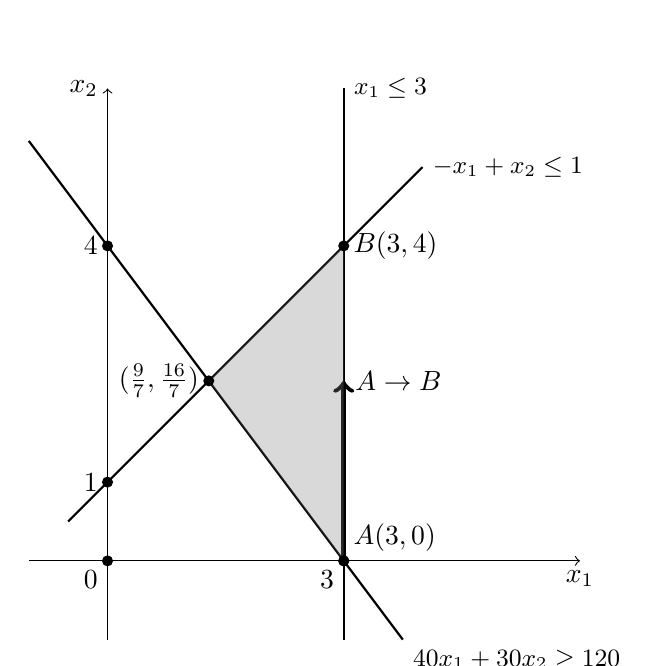
\begin{tikzpicture}
        % Draw axes
        \draw[->] (-1,0) -- (6,0) node[below] {$x_{1}$};
        \draw[->] (0,-1) -- (0,6) node[left] {$x_{2}$};
        \draw[->, line width = 0.6mm] (3,0) -- (3,2.286) node[right] {$A \to B$};

        % Constraint 1: 40x_1 + 30x_2 >= 120
        \draw[thick] (-1,5.333) -- (3.75,-1) node[below right]{\small $40 x_{1} + 30 x_{2} \geq 120$};

        % Constraint 2: x_1 <= 3
        \draw[thick] (3,-1) -- (3,6) node[right]{\small $x_{1} \leq 3$};

        % Constraint 3: -x_1 + x_2 <= 1
        \draw[thick] (-0.5,0.5) -- (4,5) node[right]{\small $-x_{1} +x_{2} \leq 1$};

        \fill[gray, opacity=0.3] (1.286,2.286) -- (3,4) -- (3,0) -- cycle;

        % Corner Points
        \fill (0,4) circle (2pt) node[left] {$4$};
        \fill (0,1) circle (2pt) node[left] {$1$};
        \fill (1.286,2.286) circle (2pt) node[left] {$(\frac{9}{7},\frac{16}{7})$};
        \fill (3,0) circle (2pt) node[below left] {$3$};
        \fill (3,0) circle (2pt) node[above right] {$A(3,0)$};
        \fill (3,4) circle (2pt) node[right] {$B(3,4)$};
        \fill (0,0) circle (2pt) node[below left] {$0$};
    \end{tikzpicture}
    \caption{Feasible Region of LP}
    \label{fig:2-feasibleregionlp}
\end{figure} 

\subsection*{(d)}
The iteration is shown in Figure \ref{fig:2-feasibleregionlp} above (thick arrow, from A to B).

\newpage

\section*{Question 3}

\begin{table}[H]
    \centering
    \begin{tabular}{c | c c | c c c c c}
        Row & & & $x_{1}$ & $x_{2}$ & $x_{3}$ & $x_{4}$ & $x_{5}$ \\ \hline 
        $R_{0}$ & & 10 & c & 2 & 0 & 0 & 0 \\ \hline
        $R_{1}$ & $x_{3}$ & 4 & a & 2 & 1 & 0 & 0 \\ 
        $R_{2}$ & $x_{4}$ & 1 & -2 & -4 & 0 & 1 & 0 \\
        $R_{3}$ & $x_{5}$ & b & -1 & 3 & 0 & 0 & 1 \\ 
    \end{tabular}
    \caption{Simplex Tableau Q3}
    \label{tab: 3-tableau1}
\end{table}

\subsection*{(a)}
Conditions on the unknowns such that current solution is \textbf{infeasible}: \\ 

\noindent We require $a \in \mathbb{R}, b < 0, c \in \mathbb{R}$.

\subsection*{(b)}
Conditions on the unknowns such that current solution is \textbf{optimal}: \\ 

\noindent We require $a \in \mathbb{R}, b \geq 0, c\geq 0$.

\subsection*{(c)}
Conditions on the unknowns such that current solution is \textbf{degenerate}: \\ 

\noindent We require $a \in \mathbb{R}, b = 0, c \in \mathbb{R}$.

\subsection*{(d)}
Conditions on the unknowns such that current solution is \textbf{optimal and there are multiple optimal solutions}: \\ 

\noindent We require $a \in \mathbb{R}, b \geq 0, c = 0$.

\subsection*{(e)}
Conditions on the unknowns such that optimal value is \textbf{unbounded}: \\ 

\noindent We require $a \leq 0, b \geq 0, c < 0$.

\newpage

\section*{Question 4}

\subsection*{(a)}
\textbf{FALSE}. At any step of the simplex method, basic variables may change, and nonbasic variables may enter or leave the basis. However, the reduced cost of a nonbasic variable may not necessarily be zero, but it will be zero for the basic variables. 

\subsection*{(b)}
\textbf{FALSE}. At the optimal tableau of the simplex method, as long as the reduced cost of a nonbasic variable is zero or positive (non-negative), the tableau is optimal. 

\subsection*{(c)}
\textbf{FALSE}. There are cases where the optimal solution may not correspond to a BFS. This occurs in \textbf{degenerate cases} or when the \textbf{feasible region is unbounded}. In these cases, the optimal solution involves non-basic variables taking non-zero values, which results in a non-BFS.

\subsection*{(d)}
\textbf{TRUE}. Since the simplex method converges to an optimal solution, it must encounter at least one BFS during any iteration that corresponds to the optimal solution. If there is an optimal solution, then there must be an optimal solution which is a BFS. 

\subsection*{(e)}
\textbf{TRUE}. The vertices correspond to the corner points of the feasible region. Since the feasible region is bounded by linear constraints, and each vertex represents a unique intersection of these constraints, there can only be a finite number of vertices, as a finite number of linear equations or inequalities can only define a finite number of intersection points.

\subsection*{(f)}
\textbf{FALSE}. If the primal linear program has an unbounded objective function value, it implies that the constraints of the dual linear program are infeasible. 

\newpage

\section*{Question 5}
The LP in Question 1 is given by: \begin{align*}
    \qquad \max \quad & 24 x_{1} + 22 x_{2} + 45 x_{3} \\ 
    \qquad \text{s.t.} \quad & 2 x_{1} + x_{2} + 3 x_{3} \leq 42 \\ 
    (\mathbb{P}) \qquad \qquad & 2 x_{1} + x_{2} + 2 x_{3} \leq 40 \\ 
    \qquad & x_{1}, x_{2}, x_{3} \geq 0
\end{align*} after removing one of the linearly dependent constraints, while keeping the tighter constraint. 

\subsection*{(a)}

The dual of the LP is given by \begin{align*}
    \min \quad & 42 p_{1} + 40 p_{2} \\ 
    \text{s.t.} \quad & 2 p_{1} + 2 p_{2} \geq 24 \\ 
    & p_{1} + p_{2} \geq 22 \\ 
    & 3 p_{1} + 2 p_{2} \geq 45 \\ 
    & p_{1}, p_{2} \geq 0
\end{align*} We can again \textbf{remove one of the linearly dependent} constraints, while keeping the tighter constraint: \begin{align*}
    \qquad \min \quad & 42 p_{1} + 40 p_{2} \\ 
    \qquad \text{s.t.} \quad & p_{1} + p_{2} \geq 22 \\ 
    (\mathbb{D})\qquad \qquad & 3 p_{1} + 2 p_{2} \geq 45 \\ 
    \qquad & p_{1}, p_{2} \geq 0
\end{align*}

\subsection*{(b)}
To find the dual optimal solution, we proceed with utilising the complementary slackness conditions. From Question 1, we have determined the optimal solution $\mathbf{x} = (x_{1}^{*}, x_{2}^{*}, x_{3}^{*}) = (0, 36, 2)$. \\ 

\noindent Using the conditions $(c_j - \mathbf{p}^{\top}\mathbf{A}_j)x_j = 0 \quad \forall j$ and $(\mathbf{a}_i^{\top}\mathbf{x}-b_i)p_i = 0 \quad \forall i$: \begin{align}
    (p_{1}^{*} + p_{2}^{*} - 22) x_{1}^{*} &= 0 \\ 
    (3 p_{1}^{*} + 2 p_{2}^{*} - 45)x_{2}^{*} &= 0 \\ 
    (2 x_{1}^{*} + x_{2}^{*} + 3 x_{3}^{*} - 42)p_{1}^{*} &= 0 \\ 
    (2 x_{1}^{*} + x_{2}^{*} + 2 x_{3}^{*} - 40)p_{2}^{*} &= 0 
\end{align} From Equations (3) and (4), we substitute the optimal solution and obtain that: \begin{align*}
    (2 x_{1}^{*} + x_{2}^{*} + 3 x_{3}^{*} - 42) &= (2 (0) + 36 + 3 (2)) = 0 \\ 
    (2 x_{1}^{*} + x_{2}^{*} + 2 x_{3}^{*} - 40) &= (2(0) + 36 + 2(2)) = 0
\end{align*} With the left coefficient of $p_{1}^{*}$ and $p_{2}^{*}$ being 0, we know that $p_{1}^{*}$ and $p_{2}^{*}$ cannot be 0. Thus to satisfy equations (1) and (2), we need $x_{1}^{*}$ and $x_{2}^{*}$ to be 0. We then have the two simultaneous equations to solve: \begin{align*}
    p_{1}^{*} + p_{2}^{*} &= 22 \\ 
    3 p_{1}^{*} + 2 p_{2}^{*} &= 45
\end{align*} This yields a solution of $p_{1}^{*} = 1$ and $p_{2}^{*} = 21$. The \textbf{dual optimal solution }is thus $(p_{1}^{*}, p_{2}^{*}) = (1, 21)$

\newpage 

\section*{Question 6}

\subsection*{(a)}
We have the primal LP \begin{align*}
    \qquad \min \quad & \mathbf{c}^{\top}\mathbf{x} \\ 
    (\mathbb{P}) \qquad \text{s.t.} \quad & \mathbf{Ax} \geq \mathbf{b} \\ 
    & \mathbf{x} \in \mathbb{R}
\end{align*} The dual is given by \begin{align*}
    \qquad \max \quad & \mathbf{p}^{\top}\mathbf{b} \\ 
    (\mathbb{D}) \qquad \text{s.t.} \quad & \mathbf{p}^{\top}\mathbf{A} = \mathbf{c}^{\top} \\
    & \mathbf{p} \geq \mathbf{0}
\end{align*}

\subsection*{(b)}
\begin{proof}
    In order to prove weak duality, we need to show that $\mathbf{c}^{\top}\mathbf{x} \geq \mathbf{p}^{\top}\mathbf{b}$. Consider a primal feasible $\mathbf{x}$ satisfying $\mathbf{Ax} \geq \mathbf{b}$ and dual feasible $\mathbf{p}^{\top}\mathbf{A} = \mathbf{c}^{\top}$. We start with one side of the equation: \begin{align*}
        \mathbf{p}^{\top}\mathbf{b} &\leq \mathbf{p}^{\top}\mathbf{Ax} \quad \text{(since } \mathbf{Ax} \geq \mathbf{b}) \\ 
        &= (\mathbf{p}^{\top}\mathbf{A})\mathbf{x} \quad \text{(by associativity)} \\ 
        &= \mathbf{c}^{\top}\mathbf{x} \quad \text{(from dual)} \qedhere
    \end{align*} 
\end{proof}

\subsection*{(c)}
The strong duality theorem states that if a linear program has an optimal solution, so does its dual and \textbf{both the optimal objective values are equal}, i.e. $\mathbf{p}^{\top}\mathbf{b} = \mathbf{c}^{\top}\mathbf{x}$. \\ 

\noindent However, if the primal $(\mathbb{P})$ is unbounded, then the dual LP is infeasible. Furthermore, if the primal LP $(\mathbb{P})$ is infeasible, then our dual LP is unbounded. 

\newpage

\section*{Question 7}
We have the LP \begin{align*}
    \min \quad & \sum_{i=1}^{n} c_i x_i \\ 
    \text{s.t.} \quad & \sum_{i=1}^{n} x_i = 1 \\ 
    & x_i \geq 0, \quad \forall i = 1, \dots , n
\end{align*}

\subsection*{(a)}

In order to find the optimal solution to the LP, we first set the most negative value of $c_i$ to be $c_{\text{min}}$. Intuitively, we can achieve the minimum objective value by \textbf{setting the variable $x_i$ corresponding to $c_{\text{min}}$ to its maximum possible value (which is 1 for all the $x_i$'s.)}, while keeping all other variables $x_i$ as small as possible, which in this case means \textbf{setting them to 0}. The optimal solution can thus be represented by the piecewise function \begin{align*}
    x_i^{*} = \begin{cases}
        1 & \quad \text{if } i = j, \; \forall i = 1, \dots , n\\ 
        0 & \quad \text{otherwise}
    \end{cases}
\end{align*} where $j$ corresponds to the index of $c_{\text{min}}$. 

\subsection*{(b)}
We can express the original LP in the more familiar notation: \begin{align*}
    \qquad \min \quad & \mathbf{c}^{\top}\mathbf{x} \\ 
    (\mathbb{P}) \qquad \text{s.t.} \quad & \sum_{i=1}^{n} x_i = 1 \\ 
    \qquad & x_i \geq 0, \; \forall i = 1, \dots, n
\end{align*} The appropriate dual is given by \begin{align*}
    \qquad \max \quad & \mathbf{p}^{\top}\mathbf{b} \\ 
    (\mathbb{D}) \qquad \text{s.t.} \quad & \mathbf{p}^{\top}\mathbf{A} \leq \mathbf{c}^{\top} \\ 
    \qquad & \mathbf{p} \in \mathbb{R}
\end{align*} \\

\noindent To find the optimal solution of the dual, we use the fact that since the primal $(\mathbb{P})$ has an optimal solution from above, then by the \textbf{strong duality theorem}, the dual \textbf{optimal objective value is equivalent to that of the primal}. We thus have: \begin{align*}
    \mathbf{p}^{\top}\mathbf{b} &= \mathbf{c}^{\top}\mathbf{x} \\ 
    \mathbf{p}^{\top} &= \mathbf{c}^{\top}\mathbf{x} \quad (\because \mathbf{b} = \mathbf{1})\\ 
    \mathbf{p} &= \mathbf{x}^{\top}\mathbf{c} \quad (\text{by transpose property})\\ 
    &= c_{\text{min}} \quad \text{(from part (a))}
\end{align*}

\end{document}
